\documentclass[a4paper,12pt]{article}

\usepackage{fancyhdr}
\lhead{\footnotesize{Project CUDC Report}}
\lfoot{\footnotesize{CS 217 Fall 2015}}
\rfoot{\footnotesize{OUNAN DING 861194909}}
\pagestyle{fancy}

\usepackage{hyperref}

\usepackage{amsmath}

% For \mathds
\usepackage{dsfont}

\usepackage{tikz}
\usetikzlibrary{patterns}

\usepackage{graphicx}

\title{Project CUDC Report}
\date{}
\author{
OUNAN DING\\
Student ID: 861194909\\
oding001@ucr.edu
}

\begin{document}

\maketitle{}

\tableofcontents{}

\section{Overview}

This report is for the final project of CS/EE-217 GPU Architecture
and Programming.
Implementations of dual contouring will be presented and analyzed.

We provide a CPU implementation written in C\texttt{++} first as our baseline,
then move on to introduce the CUDA implementations.
We will see what the bottle neck is in our CPU version,
and how we make trade off in the CUDA version to overcome that bottle neck.
A visualizer is also provided as a Blender add-on
to preview the results and check the correctness.

Finally we will provide some performance testing and detailed analysis
in the latter part of this report.

\section{Design and Implementation}

\subsection{General Overview}

In this section we will provide a general overview of dual contouring algorithm.
The architecture-independent perspectives
of this algorithm will be discussed.

The primary paper used for this project is \cite{ju2002dual}.
\cite{schaefer2002dual} also provides supplemental materials
on how to construct and solve the Quadratic Error Function(QEF).

For the first step in dual contouring, given an implicit function
such as $(x^2 + y^2 - 1)^3 - x^2y^3$ in 2D, or $x^2 + y^2 + z^2 - 1$ in 3D,
we will sample the function on a uniform grid.
Here is an example in figure \ref{fig:sampling-2d-dc},
where we sample the function $x^2 + y^2 - 1.7$.
The $0$ level set of this function is plotted as a circle of radius $1.7$.
The samples which have a negative value are drawn with solid dots.

\begin{figure}[h]
\centering
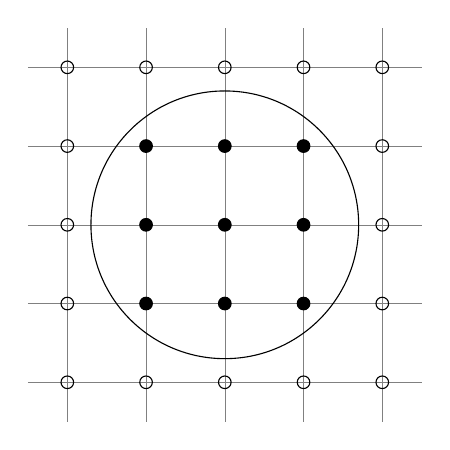
\begin{tikzpicture}

\draw[step=1, gray, very thin] (-2.5, -2.5) grid (2.5, 2.5);
\draw (0, 0) circle (1.7);

\draw (-2, -2) circle (0.08);
\draw (-1, -2) circle (0.08);
\draw (0, -2) circle (0.08);
\draw (1, -2) circle (0.08);
\draw (2, -2) circle (0.08);

\draw (-2, -1) circle (0.08);
\filldraw (-1, -1) circle (0.08);
\filldraw (0, -1) circle (0.08);
\filldraw (1, -1) circle (0.08);
\draw (2, -1) circle (0.08);

\draw (-2, 0) circle (0.08);
\filldraw (-1, 0) circle (0.08);
\filldraw (0, 0) circle (0.08);
\filldraw (1, 0) circle (0.08);
\draw (2, 0) circle (0.08);

\draw (-2, 1) circle (0.08);
\filldraw (-1, 1) circle (0.08);
\filldraw (0, 1) circle (0.08);
\filldraw (1, 1) circle (0.08);
\draw (2, 1) circle (0.08);

\draw (-2, 2) circle (0.08);
\draw (-1, 2) circle (0.08);
\draw (0, 2) circle (0.08);
\draw (1, 2) circle (0.08);
\draw (2, 2) circle (0.08);

\end{tikzpicture}
\caption{Sampling of $x^2 + y^2 - 1.7$}
\label{fig:sampling-2d-dc}
\end{figure}

Every edge which exhibits opposite signs at its ends
has a potential intersection with the $0$ level set of the function.
We highlight these edges in figure \ref{fig:intersected-edges-2d-dc}.

\begin{figure}[h]
\centering
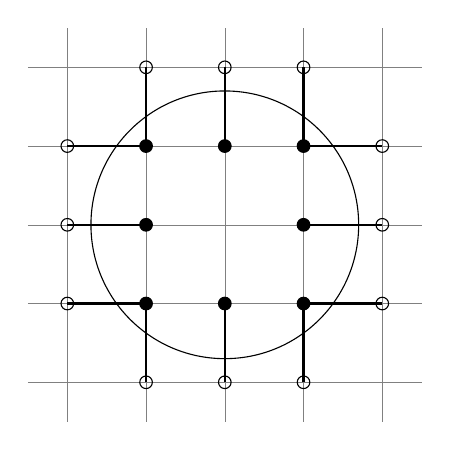
\begin{tikzpicture}
\draw[step=1, gray, very thin] (-2.5, -2.5) grid (2.5, 2.5);
\draw (0, 0) circle (1.7);

\draw (-1, -2) circle (0.08);
\draw (0, -2) circle (0.08);
\draw (1, -2) circle (0.08);

\draw (-2, -1) circle (0.08);
\filldraw (-1, -1) circle (0.08);
\filldraw (0, -1) circle (0.08);
\filldraw (1, -1) circle (0.08);
\draw (2, -1) circle (0.08);

\draw (-2, 0) circle (0.08);
\filldraw (-1, 0) circle (0.08);
\filldraw (1, 0) circle (0.08);
\draw (2, 0) circle (0.08);

\draw (-2, 1) circle (0.08);
\filldraw (-1, 1) circle (0.08);
\filldraw (0, 1) circle (0.08);
\filldraw (1, 1) circle (0.08);
\draw (2, 1) circle (0.08);

\draw (-1, 2) circle (0.08);
\draw (0, 2) circle (0.08);
\draw (1, 2) circle (0.08);

% Draw intersected edges.
\draw[thick] (-1, -2) -- (-1, -1);
\draw[thick] (0, -2) -- (0, -1);
\draw[thick] (1, -2) -- (1, -1);

\draw[thick] (-2, -1) -- (-1, -1);
\draw[thick] (1, -1) -- (2, -1);

\draw[thick] (-2, 0) -- (-1, 0);
\draw[thick] (1, 0) -- (2, 0);

\draw[thick] (-2, 1) -- (-1, 1);
\draw[thick] (-1, 1) -- (-1, 2);
\draw[thick] (0, 1) -- (0, 2);
\draw[thick] (1, 1) -- (2, 1);
\draw[thick] (1, 1) -- (1, 2);

\end{tikzpicture}
\caption{The intersected edges}
\label{fig:intersected-edges-2d-dc}
\end{figure}

The intersections of these edges can be found by a binary search.
And the gradients at the intersections
(the Hermitian data in the glossary of \cite{ju2002dual})
can be computed by finite differencing.
The result of this step is illustrated in figure \ref{fig:intersections-2d-dc}.

\begin{figure}[h]
\centering
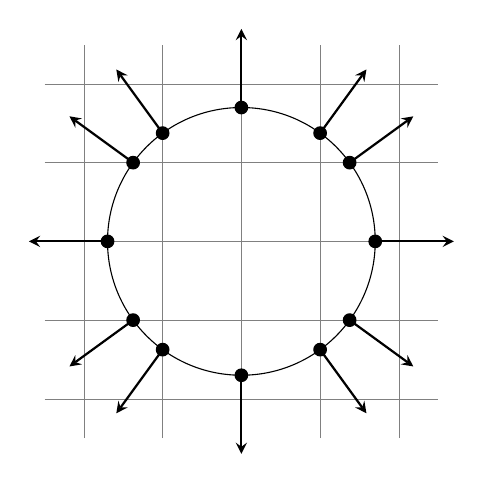
\begin{tikzpicture}
\draw[step=1, gray, very thin] (-2.5, -2.5) grid (2.5, 2.5);
\draw (0, 0) circle (1.7);

% Draw intersections.
\filldraw (-1, -1.3748) circle(0.08);
\filldraw (0, -1.7) circle(0.08);
\filldraw (1, -1.3748) circle(0.08);

\filldraw (-1.3748, -1) circle(0.08);
\filldraw (1.3748, -1) circle(0.08);

\filldraw (-1.7, 0) circle(0.08);
\filldraw (1.7, 0) circle(0.08);

\filldraw (-1.3748, 1) circle(0.08);
\filldraw (-1, 1.3748) circle(0.08);
\filldraw (0, 1.7) circle(0.08);
\filldraw (1, 1.3748) circle(0.08);
\filldraw (1.3748, 1) circle(0.08);

% Draw gradients.
\draw[->, >=stealth, thick] (-1, -1.3748) -- (-1.5882, -2.1835);
\draw[->, >=stealth, thick] (0, -1.7) -- (0, -2.7);
\draw[->, >=stealth, thick] (1, -1.3748) -- (1.5882, -2.1835);

\draw[->, >=stealth, thick] (-1.3748, -1) -- (-2.1835, -1.5882);
\draw[->, >=stealth, thick] (1.3748, -1) -- (2.1835, -1.5882);

\draw[->, >=stealth, thick] (-1.7, 0) -- (-2.7, 0);
\draw[->, >=stealth, thick] (1.7, 0) -- (2.7, 0);

\draw[->, >=stealth, thick] (-1.3748, 1) -- (-2.1835, 1.5882);
\draw[->, >=stealth, thick] (-1, 1.3748) -- (-1.5882, 2.1835);
\draw[->, >=stealth, thick] (0, 1.7) -- (0, 2.7);
\draw[->, >=stealth, thick] (1, 1.3748) -- (1.5882, 2.1835);
\draw[->, >=stealth, thick] (1.3748, 1) -- (2.1835, 1.5882);

\end{tikzpicture}
\caption{Intersections and their Hermitian data}
\label{fig:intersections-2d-dc}
\end{figure}

After the Hermitian data is ready,
the QEFs can be built as following:

\begin{eqnarray*}
E[x] & = & \sum_i {(n_i \cdot (x - p_i))^2}\\
& = & x^T A^T Ax - 2x^T A^T b + b^T b
\end{eqnarray*}

In 2D dual contouring,
each QEF can be represented by $7$ floating point numbers.
Since $A^T A$ is a $2\times 2$ symmetrical matrix, it requires $3$ floats.
The $A^T b$ is a $2\times 1$ column vector, so it requires $2$ floats.
We also store $2$ floats for the mass point,
which is a $2\times 1$ column vector and will be used in mass point projection
(see \cite{schaefer2002dual} for details about mass point projection).

We solve the QEF by computing the pseudo-inverse
as suggested in \cite{ju2002dual}.
And compute a $2\times2$ SVD for the pseudo-inverse.
This method is described in \cite{blinn2003jim}.

After solving all of the QEFs, we get all vertices of the result mesh.
We can build the topology by connecting vertices from
adjacent grid cells.

Figure \ref{fig:2d-dc-example} illustrates dual contouring results
of a heart, a squircle($x^4 + y^4 - 1$),
and the subtraction of them.

\begin{figure}[h]
\centering
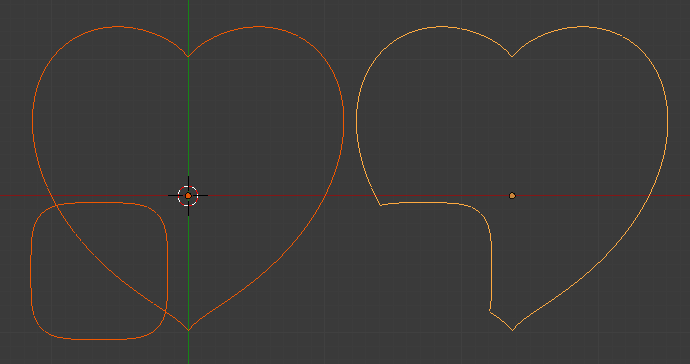
\includegraphics[width=0.9 \textwidth]{heart-squircle-subtraction.png}
\caption{2D dual contouring example}
\label{fig:2d-dc-example}
\end{figure}

\subsection{The CPU Implementation in C\texttt{++}}

There are several considerations
in our implementation of dual contouring on CPU.

First, a trivial implementation which stores the whole mesh grid
suggests a spatial complexity of $\mathcal{O}(n^2)$(or $\mathcal{O}(n^3)$
in 3D).
We do not want the memory consumption be a bottle neck,
so we do the sampling in a row by row manner.
Then only one row has to be maintained during sampling,
and one extra row has to be maintained for the topology construction
since we have to connect edges to the vertices in the previous row.
Thus the spatial complexity can be reduced to
$\mathcal{O}(n)$ in 2D(or $\mathcal{O}(n^2)$ in 3D).

Second, we think the sampling would occupy the majority time
of the whole computation(However this turns out to be \emph{false}.
See our later performance report and analysis).
So we want to reduce the computation as much as we can.
Observing that each sampling vertex has $4$ adjacent grid cells,
we can do the sampling only once, cache it in memory,
and reuse it for all adjacent grid cells.

The computing scheme is illustrated in figure \ref{fig:computing-scheme-cpp}.
Each dots indicate a sampling point.
And the dashed rectangle indicates the row we are working on.
The hatched area indicates a $4$ elements wide SIMD pack if SSE is used.

\begin{figure}[h]
\centering
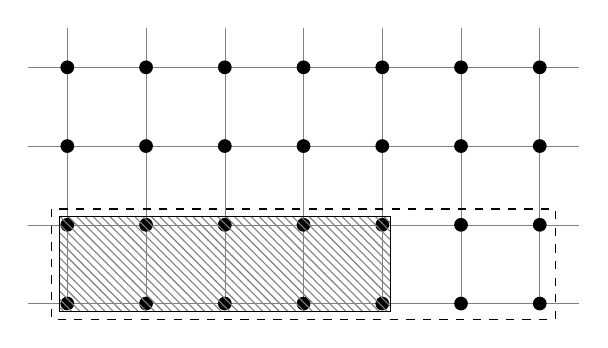
\begin{tikzpicture}
\draw[step=1, gray, very thin] (-3.5, 0) grid (3.5, 3.5);

% Draw samples.
\foreach \x in {-3, ..., 3}
{
    \foreach \y in {0, ..., 3}
        \filldraw (\x, \y) circle (0.08);
}

% Draw current row.
\draw[dashed] (-3.2, 1.2) rectangle (3.2, -0.2);

% Draw SIMD pack.
\draw[pattern=north west lines, pattern color=gray]
(-3.1, 1.1) rectangle (1.1, -0.1);

\end{tikzpicture}
\caption{The computing scheme in C\texttt{++}}
\label{fig:computing-scheme-cpp}
\end{figure}

\subsection{The CUDA Implementation}

Being similar to the CPU implementation,
we also use the row by row approach in the CUDA version
to reduce the spatial complexity.
And to utilize the high throughput of GPU we expand each row into
a tile.

In figure \ref{fig:computing-scheme-cuda} the computing scheme is illustrated.
The dashed bounding rectangle indicates a CUDA grid;
one CUDA block is drawn as solid rectangle;
and one CUDA thread is drawn as hatched rectangle.

Should we cache the sampled values like what we do in CPU implementation?
A preliminary performance test in CPU implementation
reports that the sampling occupies only $5\%$ of the whole algorithm,
while the memory access occupies almost rest of the running time.
Therefore we decide not to cache sampled values.
That is, we sacrifice some duplicated computations for less memory access.

Concretely,
every grid cell(which is mapped to a CUDA thread)
computes $4$ samples at its corner.
Then every grid vertex gets sampled for $4$ times by its adjacent cells.
In this way although duplicated computations are performed,
we can avoid the writing to the memory.

Besides, since not every grid cell have intersections and contribute
one QEF, we have to do a streaming compaction.
In a traditional implementation of streaming compaction,
prefix sum is implemented and an extra global array will be filled to
do prefix sum across blocks.
In our implementation, we use \texttt{\_\_syncthreads\_count}
to count the sum in one block,
and use atomic operations to compute the offset of each block.
Hence no extra global array is required.

\begin{figure}[h]
\centering
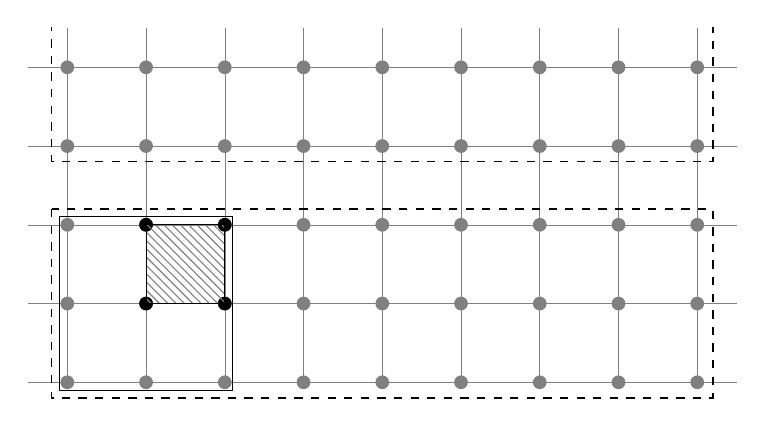
\begin{tikzpicture}
\draw[step=1, gray, very thin] (-4.5, 0) grid (4.5, 4.5);

% Draw samples.
\foreach \x in {-4, ..., 4}
{
    \foreach \y in {0, ..., 4}
        \filldraw[gray] (\x, \y) circle (0.08);
}

% Draw computing grids.
\draw[dashed] (-4.2, 2.2) rectangle (4.2, -0.2);
\begin{scope}
    \clip (-4.5, 0) rectangle (4.5, 4.5);
    \draw[dashed] (-4.2, 5.2) rectangle (4.2, 2.8);
\end{scope}

% Draw computing blocks.
\draw (-4.1, 2.1) rectangle (-1.9, -0.1);

% Draw one thread.
\filldraw (-3, 1) circle (0.08);
\filldraw (-2, 1) circle (0.08);
\filldraw (-3, 2) circle (0.08);
\filldraw (-2, 2) circle (0.08);
\draw[pattern=north west lines, pattern color=gray]
(-3, 2) rectangle (-2, 1);

\end{tikzpicture}
\caption{The computing scheme in CUDA}
\label{fig:computing-scheme-cuda}
\end{figure}

\section{Performance Test and Analysis}

All performance tests are taken on Windows 10 x86\_64,
with Visual C\texttt{++} 2013 and CUDA toolkit 7.5.
The CPU is i5 6600k @ 4.17GHz with 16 GB DDR4 RAM; the GPU is GTX 970.

The test case is to dual contour a heart equation
on the domain $[-500, 500]\times[-500, 500]$
with grid resolution of $20000$.

\subsection{The CPU Implementation in C\texttt{++}}

We use Intel's Amplifier XE to analyze the detailed time consumption
of our CPU implementation.
The total running time is 3.136 seconds.
The top-down tree of the running time is shown in table
\ref{tab:dc2-cpu-performance}.

\begin{table}[h]
\centering
\begin{tabular}{| l | l | l |}
\hline
Function Stack & CPU Time: Total & CPU Time: Self\\  \hline
\texttt{CollectIntersectionEdge2} & 40.4\% & 1.232s \\
\texttt{ConstructQEF2} & 40.1\% & 1.222s \\
\texttt{GenericDualContour2} & 12.0\% & 0.367s \\
\texttt{Sample2} & 6.7\% & 0.203s \\
\hline
\end{tabular}
\caption{Top-down tree of the running time of CPU implementation}
\label{tab:dc2-cpu-performance}
\end{table}

The bottle neck is in the gathering of intersected edges and
QEF construction, which is also a gathering operation.

By inspecting the hot spot in the source code,
we can find that about half of the time is in the memory access.
Therefore our implementation is memory bound.

Because the sampling only occupies a minority of runtime,
we can trade some computation for better memory performance.

\subsection{The CUDA Implementation}

The total running time is 0.556 seconds.
It is about 5.64x speed-up comparing with the CPU implementation.

We supply \texttt{-G} option in our kernel compilation to generate
profiling information
and use NVIDIA's Visual Profiler
to produce detailed information of running time.
It is shown in table \ref{tab:cudc2-cuda-performance}.

\begin{table}[h]
\centering
\begin{tabular}{| l | l | l |}
\hline
& \texttt{KDualContour2} & \texttt{KBuildTopology}\\  \hline
Global Memory Load Efficiency & 0\% & 82.1\%\\
Global Memory Store Efficiency & 82.1\% & 0\%\\
Shared Memory Efficiency & 23.4\% & 23.4\%\\
Branch Efficiency & 100\% & 100\%\\
\hline
\end{tabular}
\caption{Details of the running time of CUDA implementation}
\label{tab:cudc2-cuda-performance}
\end{table}

Since most of the cells do not contribute to the zero level set
of the function, so we can see the divergence does not cause serious problems.

The kernel \texttt{KDualContour2} does not read from the global memory,
and \texttt{KBuildTopology} almost does not store to the global memory,
therefore we get a 0\% in the statistics.

We also see a 82.1\% global memory load efficiency
for \texttt{KDualContour2} and 82.1\% global memory store efficiency for
\texttt{KBuildTopology}.
This memory access is to store and load the QEF indices.
Most threads either write to a consecutive memory area or never write anything.
That is, it is coalesced.

In the profiler we can see many kernel invocations.
This is because we launch the kernels \texttt{KDualContour2} and
\texttt{KBuildTopology}
in an interleaved manner.
That is, we solve QEFs for one row and construct topology for that row,
then move on to the next row and repeat the same procedure.
Too many kernel invocation from host may be a problem.
But it requires further inspection.

We also notice from the profiler that the theoretical occupation is 50\%
for the kernel \texttt{KDualContour2}.
One possible optimization is to reduce the usage of shared memory
by using some Computability 3+ features such as \texttt{\_\_shfl\_down}
to increase the threads occupation.

\section{Summary}

In this project a CUDA based 2D dual contouring on uniform grid
is implemented and analyzed.
For some memory bound applications,
we learn that there is still chance to optimize it using CUDA.
By utilizing the high throughput of GPU,
we can trade some duplicated computation for a better memory performance.

There are also many issues left for future work.
The SVD and the pseudo-inverse computation is not stable.
This will cause topology incorrectness in some cases.
Besides, for practical use in video games or other interactive applications,
an adaptive dual contouring is required.

\newpage
\addcontentsline{toc}{section}{References}
\bibliography{papers}
\bibliographystyle{alpha}

\end{document}
